\documentclass{beamer}
\beamertemplatenavigationsymbolsempty
\usepackage{amsmath, amssymb, hyperref, graphics}
\usepackage{tikz}


\title{Graph Theory Lecture 6}

\begin{document}
\begin{frame}{Second unit: Algorithms}
Some topics in Decision Maths; mostly ``easy'' points on exam.
  \begin{block}{Largely about optimization problems:}
    \begin{itemize}
    \item Kruskal and Prim's algorithms for cheapest spanning trees
    \item Dijkstra's algorithm: shortest path between two points
    \item Travelling Salesperson problem
    \end{itemize}
    \end{block}
  \begin{block}{In the real world: computers run these algorithm}
    From pure math perspective, interesting bits are:
    \begin{itemize}
    \item Proving the algorithm works as advertized
    \item Analyzing speed of algorithm -- can you go faster?
      \end{itemize}
    \end{block}


 \begin{block}{First topic: Pr\"ufer code}
    How many trees on $n$ vertices are there?
    \end{block}
\end{frame}

\begin{frame}{Two interpretations of counting trees}
\begin{block}{Count isomorphism classes of trees. ``unlabelled trees''}
\begin{itemize}
\item  This is what we do when we count isomers
\item No nice answer
\end{itemize}

\end{block}
\begin{block}{Count labelled trees on $n$ vertices}
\begin{itemize}
\item  Vertices are no longer interchangeable
\item $n!$ ways to label an unlabeled tree
  \item Symmetries mean some produce the same labelled tree
\end{itemize}
\end{block}
\begin{center}
\begin{tabular}{c|c|c|c|c|c|c|c}
n &  1 & 2 & 3 & 4 & 5 & 6 & 7 \\ \hline
Unlabelled trees &  1 & 1 & 1 & 2 & 3 & 6 & 11 \\ \hline
Labelled trees & 1 & 1 & 3 & 16 & 125 & 1296 & 16807
  \end{tabular}
\end{center}


\end{frame}




\begin{frame}{``Cayley's'' formula}
  \begin{theorem}[Borchardt 1860, Cayley 1889]
    There are $n^{n-2}$ labelled trees on $n$ vertices.
  \end{theorem}
Original proof used determinants.
  \begin{block}{Pr\"ufer code: another way to prove Cayley's formula}
Bijection between \emph{Trees} and \emph{Codes}
\begin{itemize}
\item $T_n=\{ \text{labelled trees on $n$ vertices}\}$ 
\item $C_n=\{(a_1,a_2,\dots, a_{n-2}) : a_i\in \{1,2,\dots, n\} \} $
\item Build a bijection between $T_n$ and $C_n$
\item $|C_n|=n^{n-2}$
  \end{itemize}
        \end{block}

  
  \begin{block}{Bijective Proofs}
    In combinatorics, bijective proofs often give more... 
\end{block}
  
\end{frame}

\begin{frame}{How to write down a labelled trees?}
  \begin{block}{Record the edges:}
    \begin{columns}
      \begin{column}{.3\textwidth}
\begin{center}
        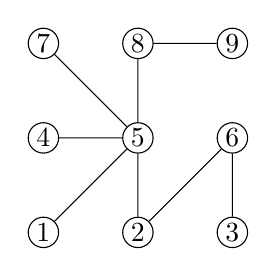
\begin{tikzpicture}[scale=1.2, every node/.style={draw, circle, fill=white, inner sep=1pt, minimum width=7pt} ]
        \node (v1) at (0,0) {$1$};
        \node (v2) at (1,0) {$2$};
        \node (v3) at (2,0) {$3$};
        \node (v4) at (0,1) {$4$};
        \node (v5) at (1,1) {$5$};
        \node (v6) at (2,1) {$6$};
        \node (v7) at (0,2) {$7$};
        \node (v8) at (1,2) {$8$};
        \node (v9) at (2,2) {$9$};
        \draw (v9)--(v8)--(v5)--(v2)--(v6)--(v3);
        \draw (v1)--(v5)--(v7);
        \draw (v4)--(v5);
    \end{tikzpicture}
\end{center}      
      \end{column}
      \begin{column}{.7\textwidth}
        \begin{center}
          Each column is an edge \\
        \begin{tabular}{c|c|c|c|c|c|c|c}
        1 & 5 & 2 & 6 & 5 & 7 & 8 & 8 \\ \hline
        5 & 2 & 6 & 3 & 4 & 5 & 9 & 5
        \end{tabular}
\end{center}
\end{column}
    \end{columns}

      \end{block}

  \begin{itemize}
  \item Records $2n-2$ numbers between 1 and $n$
  \item \emph{Many} ways of recording same tree
  \end{itemize}

  \begin{block}{Need to record the edges in a canonical way}
``Canonical'' means: without arbitrary choices
    \end{block}

\end{frame}

\begin{frame}{Pr\"ufer code: iteratively remove lowest leaf}
  \begin{enumerate}
\item Find lowest leaf $\ell$ of $T$
\item Record edge $e$ connecting it to rest of tree
\item Delete $\ell$ and $e$ to get a simpler tree $T^\prime$
\item Repeat process with $T^\prime$
  \end{enumerate}
   \begin{columns}
      \begin{column}{.3\textwidth}
\begin{center}
        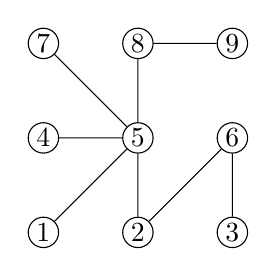
\begin{tikzpicture}[scale=1.2, every node/.style={draw, circle, fill=white, inner sep=1pt, minimum width=7pt} ]
        \node (v1) at (0,0) {$1$};
        \node (v2) at (1,0) {$2$};
        \node (v3) at (2,0) {$3$};
        \node (v4) at (0,1) {$4$};
        \node (v5) at (1,1) {$5$};
        \node (v6) at (2,1) {$6$};
        \node (v7) at (0,2) {$7$};
        \node (v8) at (1,2) {$8$};
        \node (v9) at (2,2) {$9$};
        \draw (v9)--(v8)--(v5)--(v2)--(v6)--(v3);
        \draw (v1)--(v5)--(v7);
        \draw (v4)--(v5);
    \end{tikzpicture}
\end{center}      
      \end{column}
      \begin{column}{.7\textwidth}
\begin{center}
        \begin{tabular}{r|c|c|c|c|c|c|c|c}

        Parent & \underline{5} & \underline{6} & \underline{5} & \underline{2} & \underline{5} & \underline{5} & \underline{8} & 9 \\ \hline
        Leaf   & 1 & 3 & 4 & 6 & 2 & 7 & 5 & 8 
        \end{tabular}
\end{center}
\end{column}
    \end{columns}
   \begin{block}{The underlined numbers form the Pr\"ufer code}
Non-underlined numbers are a permutation of 1-9.  Why?
   \end{block}

  \end{frame}
\begin{frame}{To see Pr\"ufer code is a bijection, construct inverse}
  \begin{block}{Given a Pr\"ufer code, how to fill in empty boxes?}
        \begin{tabular}{r|c|c|c|c|c|c|c|c}
        Parent & 5 & 6 & 5 & 2 & 5 & 5 & 8 &  \\ \hline
        Leaf   &  &  &  &  &  &  &  &  
        \end{tabular}
    \end{block}

\begin{block}{Numbers in the Pr\"ufer code were parents}
  \begin{itemize}
  \item So the numbers in Pr\"ufer code can't be leaves
  \item We deleted lowest leaf first
  \item Thus, first leaf is lowest number not in the Pr\"ufer code
  \end{itemize}
  \end{block}
\begin{block}{To reconstruct tree from code:}
  \begin{itemize}
  \item Find lowest number not used yet that's not in remaining code
  \item Delete the first column
  \item Iterate; last two numbers left are the last edge
    \end{itemize}

\end{block}

\end{frame}

\begin{frame}{Cayley's enrichment: keep track of degrees of vertices}
        \begin{tabular}{r|c|c|c|c|c|c|c|c}

        Parent & \underline{5} & \underline{6} & \underline{5} & \underline{2} & \underline{5} & \underline{5} & \underline{8} & 9 \\ \hline
        Leaf   & 1 & 3 & 4 & 6 & 2 & 7 & 5 & 8 
        \end{tabular}
        \begin{align*}
          \text{Degree of vertex $i$} & = \text{number of times $i$ appears in table} \\
          & = \text{number of times $i$ appears in Pr\"ufer code}+1
        \end{align*}


\begin{corollary}The number of labeled trees on $n$ vertices where for each $i$, vertex $i$ has degree $d_i$ is:
  $$\frac{(n-2)!}{\prod (d_i-1)!}$$
  \end{corollary}
\begin{block}{Side point: consistent with original formula}
Handshaking and multinomial formula.
\end{block}
\end{frame}


\end{document}
